% Compilar desde esta carpeta; estilo de la clase del jueves 26.
\documentclass[10pt,aspectratio=169,xcolor={dvipsnames}]{beamer}
\usepackage[utf8]{inputenc}
\usepackage[T1]{fontenc}
\usepackage{lmodern}
\usepackage[spanish,es-nodecimaldot]{babel}
\usepackage{amsmath,amssymb,bm}
\usepackage{graphicx,booktabs,tikz,listings}
\usetikzlibrary{arrows.meta,positioning,calc}
\graphicspath{{figuras/}}

% Paleta, títulos y recuadros del material DL_MRI_class.
\definecolor{fondo}{RGB}{18,49,90}
\definecolor{verde}{HTML}{087F6B}
\definecolor{naranja}{HTML}{D65324}
\setbeamercolor{normal text}{fg=fondo,bg=white}
\setbeamercolor{math text}{fg=black!75}
\setbeamercolor{structure}{fg=fondo}
\setbeamercolor{frametitle}{fg=fondo,bg=white}
\setbeamercolor{bottombox}{fg=fondo,bg=white}
\setbeamercolor{lgraybox}{fg=fondo,bg=gray!10}
\setbeamercolor{yellowbox}{fg=fondo,bg=yellow!17}
\setbeamercolor{greenbox}{fg=fondo,bg=verde!10}
\setbeamercolor{orangebox}{fg=fondo,bg=naranja!10}
\setbeamercolor{section title}{fg=fondo,bg=white}
\setbeamercolor{itemize item}{fg=fondo}
\setbeamertemplate{itemize items}[circle]
\setbeamertemplate{navigation symbols}{}
\setbeamersize{text margin left=8mm,text margin right=8mm}
\setbeamertemplate{frametitle}{\vspace{2mm}\color{fondo}\bfseries\insertframetitle\par\vspace{-2mm}\rule{\textwidth}{0.4pt}}
\setbeamertemplate{footline}{%
    \leavevmode\hbox{%
    \begin{beamercolorbox}[wd=.23\paperwidth,ht=2.5ex,dp=1ex,center]{bottombox}
        \insertshortauthor
    \end{beamercolorbox}%
    \begin{beamercolorbox}[wd=.46\paperwidth,ht=2.5ex,dp=1ex,center]{bottombox}
        \insertshorttitle
    \end{beamercolorbox}%
    \begin{beamercolorbox}[wd=.31\paperwidth,ht=2.5ex,dp=1ex,right]{bottombox}
        \insertshortdate\hspace{1.5em}\insertframenumber/\inserttotalframenumber\hspace{2ex}
    \end{beamercolorbox}}\vskip2pt}
\newcommand{\tcg}[1]{\textcolor{verde}{#1}}
\newcommand{\tcr}[1]{\textcolor{naranja}{#1}}
\newenvironment{caja}[1][lgraybox]{\begin{beamercolorbox}[sep=0.7em,wd=\linewidth]{#1}}{\end{beamercolorbox}}
\newcommand{\actividad}[2]{\begin{caja}[yellowbox]\textbf{#1}\par\smallskip #2\end{caja}}
\newcommand{\R}{\mathbb{R}}
\DeclareMathOperator*{\argmin}{arg\,min}
\lstset{language=Python,basicstyle=\ttfamily\small,keywordstyle=\color{fondo}\bfseries,
    commentstyle=\color{verde},stringstyle=\color{naranja},showstringspaces=false,
    columns=fullflexible,keepspaces=true,frame=none,aboveskip=0.5em,belowskip=0.5em}
\setbeameroption{hide notes}
% Para una versión docente intercalada, cambiar la línea anterior por:
% \setbeameroption{show notes}
\AtBeginSection[]{%
    \begin{frame}[plain]
        \vfill
        {\small APRENDIZAJE AUTOMÁTICO INICIAL\par}
        \vspace{5mm}
        {\LARGE\bfseries\insertsection\par}
        \vspace{3mm}{\color{naranja}\rule{0.25\textwidth}{1.2pt}}
        \vfill
    \end{frame}}

\title[Clase 14]{\bfseries Perceptrón multicapa}
\subtitle{Componer capas para aprender relaciones no lineales}
\author[E. Cueva]{Evelyn Cueva J.}
\institute{Aprendizaje Automático Inicial · Ciencia de Datos}
\date[1 dic. 2026]{Martes 1 de diciembre de 2026}

\begin{document}
\begin{frame}[plain]
    \vspace{6mm}{\small CLASE 14\par}\vspace{6mm}
    {\LARGE\bfseries\inserttitle\par}\vspace{3mm}
    {\color{fondo}\rule{0.92\textwidth}{1pt}}\par
    {\large\insertsubtitle\par}\vspace{8mm}
    \insertauthor\par\smallskip{\small\insertinstitute\par}\vspace{3mm}
    {\small\insertdate\par}\vfill
\end{frame}
\begin{frame}{Del clasificador lineal a una red multicapa}
\begin{itemize}
\item El lunes aprendimos a producir probabilidades y medir errores de clasificación.
\item Hoy preguntamos qué ocurre cuando la frontera necesaria no es una recta.
\item Compondremos capas y elegiremos la salida según la tarea.
\end{itemize}\begin{caja}[yellowbox]
¿Basta con entrenar durante más épocas si la arquitectura no puede representar el patrón?
\end{caja}

\note{}
\end{frame}

\begin{frame}{Objetivos y ruta de trabajo}
\begin{itemize}
\item Identificar entrada, capas ocultas y salida.
\item Explicar por qué las activaciones no lineales cambian la capacidad del modelo.
\item Configurar un MLP para regresión, clasificación binaria y multiclase.
\item Evaluar el aprendizaje con datos separados del entrenamiento.
\end{itemize}
\note{}
\end{frame}

\section{Arquitectura: componer transformaciones}
\begin{frame}{Una frontera lineal tiene límites}
\centering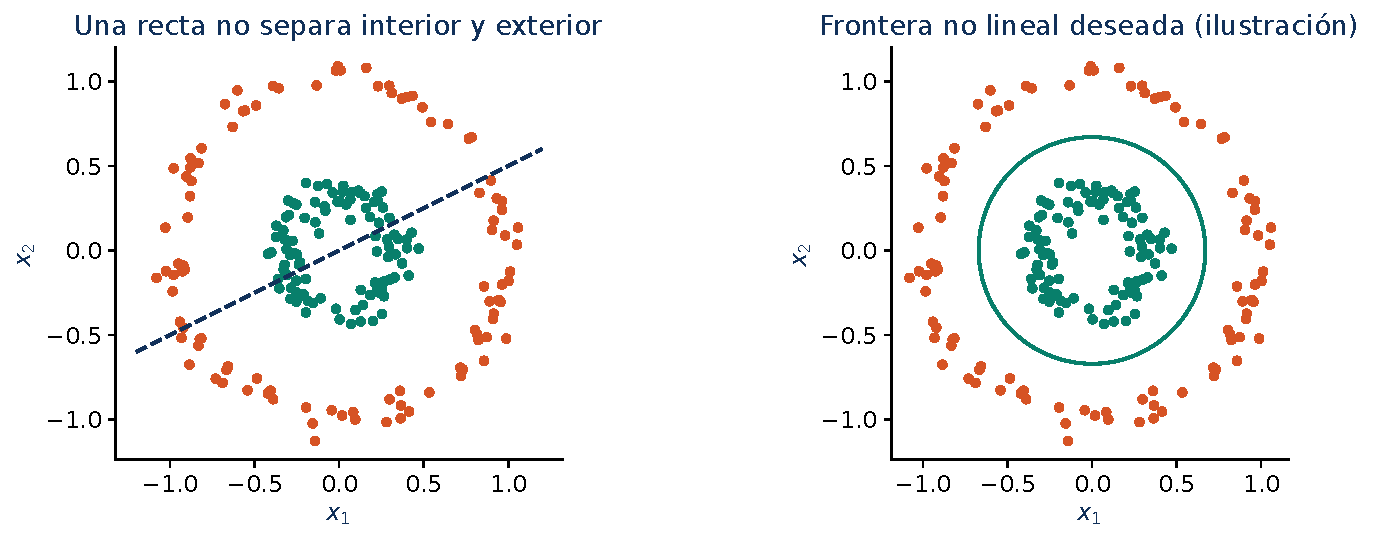
\includegraphics[width=\linewidth,height=4cm,keepaspectratio]{circulos.pdf}\par\medskip
aggedright\small Los datos interiores y exteriores no pueden separarse con una única recta. La circunferencia es una frontera deseada, no un ajuste entrenado.
\note{}
\end{frame}

\begin{frame}{Capas: de las entradas a una representación}

\centering
\begin{tikzpicture}[>=Latex,neuron/.style={circle,draw=fondo,fill=verde!10,minimum size=6mm},x=2.3cm,y=0.8cm]
\foreach \i in {1,2} {\node[neuron] (i\i) at (0,\i) {$x_\i$};}
\foreach \j in {1,2,3,4} {\node[neuron] (h\j) at (1,\j-1) {};}
\node[neuron,fill=naranja!15] (o) at (2,1.5) {$\hat y$};
\foreach \i in {1,2} {\foreach \j in {1,2,3,4} {\draw[->,fondo!45] (i\i)--(h\j);}}
\foreach \j in {1,2,3,4} {\draw[->,fondo!45] (h\j)--(o);}
\node at (0,-0.7) {Entrada: 2};\node at (1,-0.7) {Oculta: 4};\node at (2,-0.7) {Salida: 1};
\end{tikzpicture}\par\bigskip\raggedright
Cada neurona oculta combina las entradas, añade un sesgo y aplica una activación.
\par\medskip La capa de entrada representa los datos; aquí no tiene parámetros entrenables.
\note{Dibujar un sesgo en pizarra para una neurona, sin recargar todas las conexiones. Activación no significa una decisión binaria de encendido: puede ser un valor continuo.}
\end{frame}

\begin{frame}{La red es una composición de funciones}

\[\bm h=\sigma(W_1^\top\bm x+\bm b_1),\qquad
\hat{\bm y}=g(W_2^\top\bm h+\bm b_2).\]
\begin{caja}[greenbox]
Dentro de cada neurona: suma ponderada. Entre capas: composición de transformaciones.
\end{caja}
\[\bm x\in\R^2,\quad W_1\in\R^{2\times4},\quad
\bm h\in\R^4,\quad W_2\in\R^{4\times1}.\]
La activación oculta $\sigma$ y la de salida $g$ cumplen papeles diferentes.
\note{}
\end{frame}

\begin{frame}{Varias capas lineales siguen siendo un modelo afín}

Si omitimos las activaciones no lineales:
\[\bm h=W_1^\top\bm x+\bm b_1,\qquad
\hat{\bm y}=W_2^\top\bm h+\bm b_2.\]
Sustituir da:
\[\hat{\bm y}=(W_1W_2)^\top\bm x+W_2^\top\bm b_1+\bm b_2.\]
\begin{caja}[yellowbox]Añadir capas afines sin no linealidad no crea una familia de funciones más expresiva.\end{caja}
\note{}
\end{frame}

\begin{frame}{De bisagras ReLU a una aproximación curva}
\centering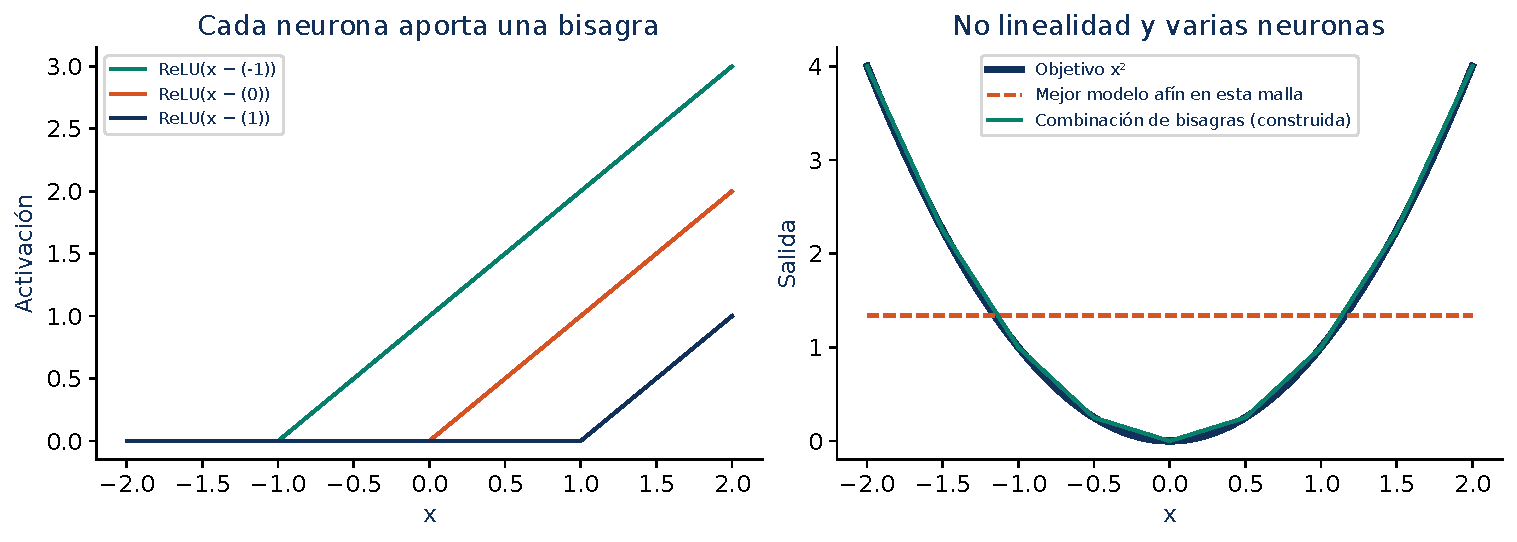
\includegraphics[width=\linewidth,height=4cm,keepaspectratio]{relu_cuadrado.pdf}\par\medskip
aggedright\small Ejemplo construido con pesos conocidos: varias bisagras permiten una aproximación por tramos de una curva.
\note{La curva verde es interpolación lineal construida, no un resultado de entrenamiento. Un MLP aprende los pesos, sesgos y posiciones de quiebre a partir de ejemplos. Más capacidad no garantiza que el entrenamiento encuentre un buen ajuste.}
\end{frame}

\begin{frame}{¿Cuántos parámetros aprende la red?}

Una capa densa de $n_{\rm entrada}$ a $n_{\rm salida}$ aprende:
\[n_{\rm entrada}n_{\rm salida}+n_{\rm salida}
=(n_{\rm entrada}+1)n_{\rm salida}.\]
\begin{caja}Red $2\to4\to1$:
\[(2+1)4+(4+1)1=12+5=17.\]
Los pesos son las conexiones; los sesgos pertenecen a las neuronas de cada capa densa.
\end{caja}
\actividad{Calcula}{¿Cuántos parámetros tiene una red $6\to12\to6\to3$?}
\note{Respuesta: 84+78+21=183. La capa de entrada no añade parámetros.}
\end{frame}

\section{Del modelo matemático a Keras}
\begin{frame}{Framework y API: qué automatizan}
\begin{itemize}
\item TensorFlow proporciona cálculo con tensores y diferenciación automática.
\item La API Keras permite declarar capas, pérdida y optimizador.
\item \texttt{Sequential}: encadena capas; \texttt{Dense}: capa completamente conectada.
\item \texttt{compile}: configura el entrenamiento; \texttt{fit}: ejecuta las actualizaciones.
\end{itemize}
\note{Los notebooks usan tensorflow.keras, no scikit-learn como framework de redes. Scikit-learn se usa para datos, particiones, escalado y métricas. No confundir compile de Keras con compilar la presentación.}
\end{frame}

\begin{frame}{Elegir la salida antes de entrenar}
\centering\small
\begin{tabular}{llll}\toprule
Tarea & Última capa & Pérdida & Etiquetas\\\midrule
Regresión escalar & 1, lineal & MSE & Reales\\
Clasificación binaria & 1, sigmoide & BCE & 0 o 1\\
Multiclase & $K$, softmax & CE categórica & One-hot\\\bottomrule
\end{tabular}\par\bigskip\raggedright
Las capas ocultas pueden ser similares; la tarea decide la salida y la pérdida.
\par\medskip Para etiquetas enteras multiclase: entropía cruzada categórica dispersa.
\note{}
\end{frame}

\begin{frame}[fragile]{Regresión: una red para datos curvos}
\begin{lstlisting}
model = Sequential([
    Input(shape=(1,)),
    Dense(8, activation="tanh"),
    Dense(1, activation="linear")
])
model.compile(optimizer=SGD(learning_rate=0.01),
              loss=MeanSquaredError())
history = model.fit(X_train, y_train, epochs=200,
                    batch_size=16,
                    validation_data=(X_val, y_val))
\end{lstlisting}

\note{Adaptación de 14-1: comparar con una sola Dense lineal. No afirmar que una neurona ReLU oculta basta para una parábola. Importar Sequential, Input, Dense, SGD y MeanSquaredError como en el notebook. Los datos deben separarse previamente.}
\end{frame}

\begin{frame}{Actividad de regresión: arquitectura o entrenamiento}
\begin{itemize}
\item Notebook 14-1: empezar con la relación lineal y una salida lineal.
\item Pasar a los datos cuadráticos y conservar el modelo: observar su limitación.
\item Comparar 1, 4 y 8 neuronas ocultas con activación tanh o ReLU.
\item Mantener partición y semilla; registrar pérdida de entrenamiento y validación.
\end{itemize}
\note{El cuaderno original usa Dense(1, relu) seguida de Dense(1, linear). Una sola bisagra tiene poca capacidad para aproximar una parábola en un intervalo simétrico. Más épocas no resuelven esa limitación por sí solas.}
\end{frame}

\begin{frame}[fragile]{Clasificación binaria: representar una frontera curva}
\begin{lstlisting}
model = Sequential([
    Input(shape=(2,)),
    Dense(4, activation="tanh"),
    Dense(1, activation="sigmoid")
])
model.compile(optimizer=SGD(learning_rate=0.1),
              loss=BinaryCrossentropy(),
              metrics=["accuracy"])
history = model.fit(X_train, y_train, epochs=200,
                    validation_data=(X_val, y_val))
\end{lstlisting}

\note{14-2: comparar datos make_blobs y make_circles. Corregir en una copia loss=BinaryCrossentropy por loss=BinaryCrossentropy(): se necesita una instancia. La tasa del ejemplo original es 0.5; aquí 0.1 es una configuración inicial para experimentar, no un óptimo garantizado.}
\end{frame}

\begin{frame}[fragile]{Multiclase: conservar softmax, añadir representación}
\begin{lstlisting}
model = Sequential([
    Input(shape=(2,)),
    Dense(8, activation="relu"),
    Dense(3, activation="softmax")
])
model.compile(optimizer=SGD(learning_rate=0.1),
              loss=CategoricalCrossentropy(),
              metrics=["accuracy"])
history = model.fit(X_train, Y_train, epochs=100,
                    validation_data=(X_val, Y_val))
\end{lstlisting}

\note{14-3 contiene únicamente Dense(3, softmax), sin capa oculta: es un punto de comparación lineal multiclase. La diapositiva muestra una extensión MLP. Y_train e Y_val son etiquetas one-hot; los nombres deben crearse al separar los datos.}
\end{frame}

\section{Caso práctico y evaluación}
\begin{frame}{Caso Pokémon: formular el problema}
\begin{itemize}
\item Notebook 14-4: predecir Stage a partir de seis características numéricas.
\item Entradas: Attack, Defense, Speed, Sp. Atk, Sp. Def y HP.
\item Red propuesta en el cuaderno: 6 entradas, capas ocultas de 12 y 6, tres salidas softmax.
\item Inspeccionar clases, faltantes y duplicados antes de entrenar.
\end{itemize}
\note{El CSV se descarga desde una URL en el cuaderno. Si se prepara una sesión sin conexión, obtener antes una copia local conservando su procedencia. Verificar que Stage tiene efectivamente tres clases válidas y codificarlas explícitamente; no usar Name como entrada.}
\end{frame}

\begin{frame}[fragile]{Separar antes de escalar: evitar fuga de información}
\begin{lstlisting}
X_train, X_temp, y_train, y_temp = train_test_split(
    X, y, test_size=0.4, stratify=y, random_state=42)
X_val, X_test, y_val, y_test = train_test_split(
    X_temp, y_temp, test_size=0.5,
    stratify=y_temp, random_state=42)
scaler = StandardScaler().fit(X_train)
X_train = scaler.transform(X_train)
X_val = scaler.transform(X_val)
X_test = scaler.transform(X_test)
\end{lstlisting}

\note{Adaptación de 14-4 y 15: los originales ajustan el escalador antes de dividir. Partir desde la matriz numérica sin escalar y las etiquetas enteras, luego codificar one-hot. Separación estratificada requiere suficientes ejemplos por clase.}
\end{frame}

\begin{frame}{Entrenamiento, validación y prueba tienen papeles distintos}
\begin{caja}[greenbox]
Entrenamiento: ajustar pesos. Validación: elegir arquitectura e hiperparámetros. Prueba: evaluación final.
\end{caja}
\begin{itemize}
\item Cambiar una decisión por experimento y registrar semilla, arquitectura, tasa y épocas.
\item No seleccionar el modelo mirando repetidamente el conjunto de prueba.
\item Comparar exactitud, matriz de confusión y desempeño por clase.
\end{itemize}
\note{}
\end{frame}

\begin{frame}{Leer la matriz de confusión}
\centering
\begin{tabular}{lccc}\toprule
Real $\backslash$ predicha & Clase 0 & Clase 1 & Clase 2\\\midrule
Clase 0 & 12 & 2 & 1\\Clase 1 & 3 & 10 & 2\\Clase 2 & 0 & 1 & 14\\\bottomrule
\end{tabular}\par\bigskip\raggedright
Ejemplo ilustrativo: exactitud $=(12+10+14)/45=0.8$.
\actividad{Discute}{¿Entre qué clases se concentra el error? ¿La exactitud global cuenta toda la historia?}
\note{}
\end{frame}

\begin{frame}{Verificación y resumen}
\begin{itemize}
\item Una red compone capas; sin activaciones no lineales, varias capas afines colapsan en una.
\item La arquitectura controla capacidad; el entrenamiento busca sus parámetros.
\item La tarea determina la capa de salida y su pérdida.
\item El miércoles: cómo se calculan los gradientes de todas las capas y cómo evitar sobreajuste.
\end{itemize}
\note{Preguntar qué significa que loss de entrenamiento baje y val_loss suba. Lectura previa de Clase14.pdf: video de retropropagación del aula virtual; la guía no entrega aquí una URL para reproducir.}
\end{frame}

\end{document}
